\documentclass[11pt,a4paper]{article}

\usepackage[margin=2.4cm]{geometry}
\usepackage[T1]{fontenc}
\usepackage{lmodern}
\usepackage{microtype}
\usepackage{amsmath,amssymb}
\usepackage{booktabs}
\usepackage{tabularx}
\usepackage{enumitem}
\usepackage{caption}
\usepackage{xcolor}
\usepackage{tikz}
\usetikzlibrary{arrows.meta,positioning,fit,backgrounds}
\usepackage[hidelinks]{hyperref}

\setlist{itemsep=2pt,topsep=4pt}
\newcommand{\code}[1]{\texttt{#1}}
\newcommand{\vect}[1]{\mathbf{#1}}

\title{Language-Guided Goals on a Frozen Gaussian Splat:\\
Embedding and Querying Semantic Features (Phases 0--4)}
\author{Suhan --- Team Radiance, Department of Computer Science and Engineering,\\University of Moratuwa}
\date{6 October 2026}

\begin{document}
\maketitle

\begin{abstract}
SOUS-VIDE/FiGS trains visuomotor drone policies inside a 3D Gaussian Splat (3DGS) reconstruction of a real room.
This report describes how we attach open-vocabulary semantic features to such a splat \emph{after} it has been
trained, without modifying it, so that a free-text phrase (``red tool chest'') resolves offline to a 3D goal and
a collision-checked approach point that becomes the final waypoint of a flight course. Two backends produce the
same per-Gaussian feature table: a training-free \emph{lift} that averages 2D CLIP and DINOv2 features onto
Gaussians through their alpha-blending weights, and \emph{FMGS}, a multi-resolution hash-grid feature field
trained against the frozen splat by differentiable rendering. On the 532{,}361-Gaussian \emph{backroom} scene the
lift localises all five development queries (errors 0.02--0.38\,m) and FMGS four of five, trained in 31.4\,min
within an 8\,GB GPU. We document the method, the system integration in the Galley web console, the engineering
problems met on an RTX~2080 (gsplat's channel limits, tiny-cuda-nn launch limits, allocator contention and fp16
overflow) and their fixes, and the evaluation planned for Phase~5.
\end{abstract}

\tableofcontents
\newpage

%=====================================================================
\section{Introduction}
%=====================================================================

The project's aim is \emph{language-guided goals for simulation-trained visuomotor drone policies}. FiGS turns a
phone capture of a room into a Gaussian splat; a course (a list of keyframes) is flown by an expert controller in
the splat's photo-realistic renders, and those flights train the SV-Net visuomotor student. Today, courses are
drawn by hand. The semantics work lets an operator \emph{name} a target instead: the system finds the object in
3D and appends an approach point to the course.

Three requirements shaped the design:
\begin{enumerate}
  \item \textbf{The splat is frozen.} Every course, cached render and trained policy depends on the splat's
        exact Gaussians. Semantics must be added on top, never by retraining the splat.
  \item \textbf{Open vocabulary.} No object list or manual labels: any phrase CLIP understands should be
        queryable. Hand-placed annotations are used only to \emph{score} results.
  \item \textbf{One 8\,GB GPU, offline queries.} Feature construction runs once per splat on an RTX~2080;
        queries run on the CPU in under a second so they never compete with simulation jobs.
\end{enumerate}

\paragraph{Related work.} LERF~\cite{lerf} distils multi-scale CLIP features into a NeRF and defines the
relevancy score we use. Feature-splatting methods attach features to Gaussians instead of a NeRF:
FMGS~\cite{fmgs} trains a hash-grid feature field queried at Gaussian centres and supervised by rendered
feature maps, with DINO features and a pixel-alignment loss sharpening CLIP's coarse maps. Training-free
approaches such as Occam's LGS~\cite{occam} and LUDVIG~\cite{ludvig} instead \emph{lift} 2D features onto
Gaussians as blend-weighted averages. We implement one of each family on identical inputs so that Phase~5 can
compare them fairly.

%=====================================================================
\section{System overview}
%=====================================================================

Figure~\ref{fig:pipeline} shows the pipeline. Both backends consume the same frozen splat, refined cameras and
cached teacher features, and write the same table; everything downstream (query worker, splat editor, course
hand-off, evaluation) is backend-agnostic.

\begin{figure}[ht]
\centering
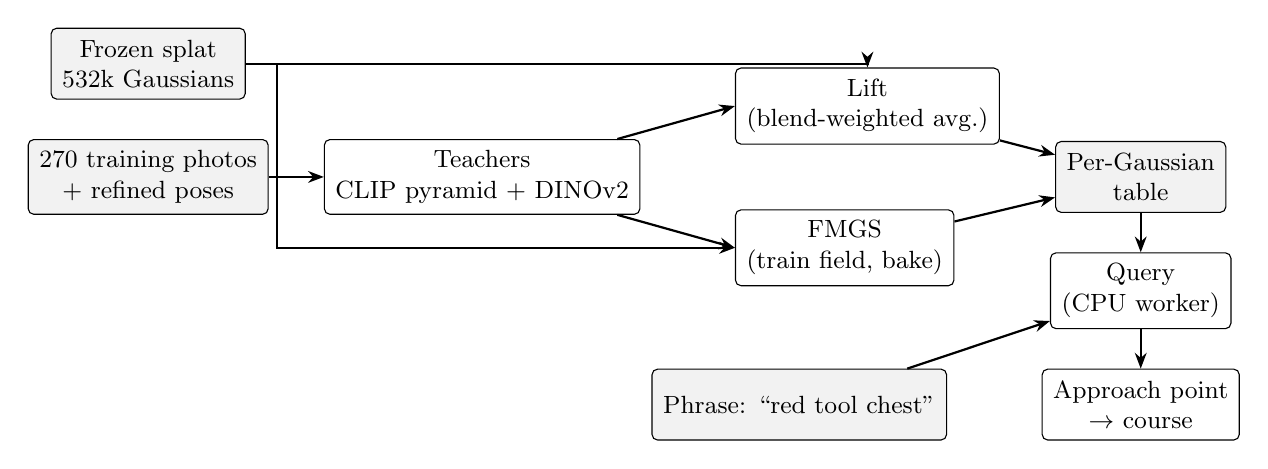
\begin{tikzpicture}[
  node distance=5mm and 7mm,
  box/.style={draw, rounded corners=2pt, align=center, font=\small, minimum height=9mm, inner sep=4pt, fill=white},
  data/.style={box, fill=gray!10},
  arr/.style={-{Stealth[length=2mm]}, thick}]
  \node[data] (splat) {Frozen splat\\532k Gaussians};
  \node[data, below=of splat] (imgs) {270 training photos\\+ refined poses};
  \node[box, right=of imgs] (teach) {Teachers\\CLIP pyramid + DINOv2};
  \node[box, right=12mm of teach, yshift=9mm] (lift) {Lift\\(blend-weighted avg.)};
  \node[box, right=12mm of teach, yshift=-9mm] (fmgs) {FMGS\\(train field, bake)};
  \node[data, right=of lift, yshift=-9mm] (table) {Per-Gaussian\\table};
  \node[box, below=of table] (query) {Query\\(CPU worker)};
  \node[box, below=of query] (course) {Approach point\\$\rightarrow$ course};
  \node[data, left=12mm of course] (text) {Phrase: ``red tool chest''};
  \draw[arr] (splat) -| (lift);
  \draw[arr] (splat.east) -- ++(4mm,0) |- (fmgs.west);
  \draw[arr] (imgs) -- (teach);
  \draw[arr] (teach) -- (lift.west);
  \draw[arr] (teach) -- (fmgs.west);
  \draw[arr] (lift) -- (table);
  \draw[arr] (fmgs) -- (table);
  \draw[arr] (table) -- (query);
  \draw[arr] (text) -- (query);
  \draw[arr] (query) -- (course);
\end{tikzpicture}
\caption{From a frozen splat to a flyable goal. Grey boxes are data; white boxes are processing steps.}
\label{fig:pipeline}
\end{figure}

\begin{table}[ht]
\centering\small
\begin{tabularx}{\linewidth}{@{}l>{\raggedright\arraybackslash}X l@{}}
\toprule
Phase & What it added & State \\
\midrule
0 & Environment (OpenCLIP, DINOv2 in the pinned FiGS stack), pose check, gsplat probes & done, 5 Oct \\
1 & Teacher features, lift backend, CLI query & done, 5/5 dev queries \\
2 & Galley backend, CPU query worker & done, warm query $\approx$0.74\,s \\
3 & Splat editor: query, highlight, send to course, fly & done \\
4 & FMGS backend (trained feature field) & done, gate passed 6 Oct \\
5 & Evaluation and comparison (two scenes, frozen query set) & next \\
6 & Instruction $\rightarrow$ semantic course $\rightarrow$ SV-Net & planned \\
\bottomrule
\end{tabularx}
\caption{Phases of the semantics work.}
\end{table}

%=====================================================================
\section{Inputs: the frozen splat and its cameras}
%=====================================================================

The \emph{backroom} scene is a nerfstudio \code{splatfacto} run (30{,}000 steps): 532{,}361 Gaussians, each with
centre $\vect{x}_i$, rotation, scale, opacity $o_i$ and colour, and 270 training views (30 more held out).

\paragraph{Refined poses.} Splatfacto jointly optimises a small SE(3) correction per training camera, but applies
it only in training mode. We apply it explicitly (\code{cameras.optimized\_c2w}). On backroom the refined poses
render the training images at 31.68\,dB PSNR versus 27.46\,dB for the raw poses (+4.22\,dB, every sampled view
better); corrections average 4.1\,mm and 0.11\textdegree{} (up to 39\,mm and 2\textdegree). Features projected
through raw poses would land up to 4\,cm off, so both backends use the refined poses.

\paragraph{Rendering features.} We render arbitrary per-Gaussian features with gsplat~1.0.0's rasteriser. Its
forward kernel accepts up to 512 channels but its \emph{backward} kernel only up to 32, so any feature tensor that
requires gradients is rendered in 32-channel chunks (\code{render.GRAD\_CHUNK}).

%=====================================================================
\section{Teacher features (Phase 1)}
%=====================================================================

Each photo is converted once into two dense 2D feature maps, cached as fp16 (1.3\,GB for backroom; 31\,min for
300 frames on the RTX~2080).

\paragraph{CLIP pyramid.} Following LERF, we use OpenCLIP ViT-B/16 (LAION-2B, 512-d). For each of 7 scales
$s \in [0.05, 0.5]$ of the image's short side, square crops of side $s\cdot\min(H,W)$ slide with half-crop
stride; each crop is resized to 224\,px and embedded, giving one unit vector per crop centre. Each scale's grid is
resampled onto one common grid ($\approx 71\times40$ cells tiling the image evenly) and the scales are averaged,
as FMGS does. About 3{,}500 crops per frame.

\paragraph{DINOv2.} ViT-S/14 patch tokens (384-d) on the image resized to multiples of 14 ($\approx 64\times36$).
DINO features carry no language but delineate objects sharply, which the CLIP pyramid does not.

%=====================================================================
\section{Backend 1: the lift (training-free)}
%=====================================================================

For Gaussian $i$, teacher map $F_v$ of view $v$ (upsampled to the render size) and the Gaussian's alpha-blending
weight $w_i(v,p)$ at pixel $p$:
\begin{equation}
  \vect{f}_i \;=\; \frac{\sum_{v,p} w_i(v,p)\, F_v(p)}{\sum_{v,p} w_i(v,p)} .
\end{equation}
Because rendering is linear in the features, the numerator equals the gradient of
$\sum_p \langle \mathrm{render}(\vect{f}), F_v\rangle$ at $\vect{f}=0$, and the denominator the gradient of
$\sum_p \mathrm{render}(\vect{1})$. The lift is therefore two backward passes per view, with no optimisation
(29 rendering passes per image in 32-channel chunks). Phase~0 verified these identities numerically on the
installed gsplat. On backroom the lift took 3\,min\,11\,s and saw 531{,}951 of 532{,}361 Gaussians; the
remainder have weight 0 and are treated as \emph{unseen} everywhere downstream.

%=====================================================================
\section{Backend 2: FMGS on a frozen splat (Phase 4)}
%=====================================================================

\subsection{Feature field}
FMGS represents semantics not as one vector per Gaussian but as a function of 3D position. Centres are
normalised into the scene's 1st--99th percentile box (padded 5\,\%) and encoded by an Instant-NGP multi-resolution
hash grid: 24 levels with resolutions growing geometrically from 16 to 512, $2^{20}$ table entries per level and 8
features per level, a 192-d encoding. Two MLP heads (2 hidden layers of 256 ReLU units) map it to a 512-d CLIP
vector and a 384-d DINO vector. Encoding and heads are tiny-cuda-nn modules (fp16 compute); the field has
113.5\,M parameters.

\paragraph{Deviation on sm\_75.} tiny-cuda-nn on the RTX~2080 refuses to launch any 192-d hash grid
(``invalid configuration argument'') at any table size or point count, while every grid up to 96 dimensions runs.
We therefore build the 24 levels as two consecutive 12-level grids (\code{FieldConfig.split = 2}), concatenated
in level order. Capacity is identical; only the second grid's base resolution is rounded to an integer, so the
ladder runs 16$\rightarrow$84 and 98$\rightarrow$512 instead of one 16$\rightarrow$512 ladder (every level within
1\,\%). This is recorded with each trained field and reported as a deviation from FMGS.

\subsection{Training against the frozen splat}
We use a standalone trainer (\code{fmgs/train.py}) rather than an \code{ns-train} plugin: since the splat is
frozen, training needs only cameras and teacher maps, and sharing the lift's cameras and rendering path keeps the
comparison fair. Each of 4{,}200 steps:
\begin{enumerate}
  \item Draw a training view at random (refined pose), feature resolution $480\times270$.
  \item Take the \emph{trainable subset} --- the most opaque 40\,\% of Gaussians (212{,}944), chosen once --- and
        keep those whose centre projects into the image (10\,\% margin): median 66{,}563 per view, at most
        140{,}374.
  \item Evaluate the field at their centres $\rightarrow$ 896 values per Gaussian.
  \item Render the features with gsplat (28 chunks of 32 channels) and divide by the rendered alpha, so that
        omitting the other 60\,\% of Gaussians does not darken the maps.
  \item Compute the loss against the view's teacher maps, upsampled to $480\times270$, on pixels with rendered
        alpha $\geq 0.5$ (set $M$):
  \begin{equation}
    \mathcal{L} = 0.2\,\mathcal{L}_{\mathrm{CLIP}} + 0.8\,\mathcal{L}_{\mathrm{DINO}} + 0.01\,\mathcal{L}_{\mathrm{PA}},
  \end{equation}
  with $\mathcal{L}_{\mathrm{CLIP}}$ a Huber loss ($\delta=1.25$) and $\mathcal{L}_{\mathrm{DINO}}$ a squared
  error, both means over $M$ and channels, and the pixel-alignment term (our reading of FMGS)
  \begin{equation}
    \mathcal{L}_{\mathrm{PA}} = \operatorname*{mean}_{(p,q)} \bigl|\cos(\hat c_p, \hat c_q) - \cos(d_p, d_q)\bigr| ,
  \end{equation}
  over 4{,}096 sampled pixels $p$ and their $3\times3$ neighbours $q$ at dilation 2, where $\hat c$ is the rendered
  CLIP map and $d$ the fixed DINO teacher. It asks rendered CLIP to relate neighbouring pixels the way DINO does,
  transferring DINO's object boundaries to CLIP.
  \item Back-propagate through the rasteriser into the field only; Adam with learning rate $10^{-2}\rightarrow10^{-3}$
        (exponential), $\epsilon = 10^{-15}$ (LERF's hash-field settings).
\end{enumerate}
The Gaussians are detached tensors that never enter the optimiser. As proof, the gate checksums the Gaussian
parameters and the checkpoint file before and after training.

\subsection{Baking}
After training, the field is evaluated once at all 532{,}361 centres and each row is normalised to unit length,
producing the same table as the lift. Rows of Gaussians no training camera saw are marked unseen, using the lift's
blend weights for the same checkpoint. The field itself is kept (\code{field.pt}) because, unlike the lift, it can
answer arbitrary 3D points.

\subsection{\texorpdfstring{Making it fit in 8\,GB, and keeping fp16 stable}{Making it fit in 8 GB, and keeping fp16 stable}}
\label{sec:engineering}
The first full run failed with \code{CUDA\_ERROR\_OUT\_OF\_MEMORY} inside tiny-cuda-nn's backward pass. A per-stage
profile on the worst view (140k Gaussians) showed live PyTorch tensors peaking at only 5.9\,GB; the failure came
from two allocators sharing one GPU. PyTorch's caching allocator held 1--3\,GB of free but fragmented blocks that
tiny-cuda-nn's own \code{cuMemCreate} arena could not use. The fixes, none of which change the method:
\begin{itemize}
  \item PyTorch's allocator runs with \emph{expandable segments}; without them even a $2^{19}$ table failed.
  \item tiny-cuda-nn's \code{RuntimeError} is recognised as out-of-memory. A failing step is retried once with the
        cache emptied and the same random state; a second failure walks the planned fallback ladder
        ($2^{19}$ table $\rightarrow$ half the visible Gaussians $\rightarrow$ B-lite).
  \item Shorter tensor lifetimes, and losses that no longer keep full-map intermediates for backward (identical
        values and gradients to $10^{-14}$).
\end{itemize}

With memory fixed, training diverged to NaN at step 11, exposing a precision problem. tiny-cuda-nn receives the
gradient of its fp16 outputs already cast to fp16, and applies its $\times128$ loss scale only afterwards. The CLIP
term is about four orders of magnitude smaller than the DINO term, so its gradients ($\sim10^{-8}$) underflowed:
only 1--2\,\% were non-zero and the CLIP head barely learned. Pixel alignment then normalised near-zero CLIP
vectors, whose gradient scales as $1/\lVert\hat c\rVert$, producing per-Gaussian gradients of $2.25\times10^4$
that overflowed fp16. Two numerical guards fixed it:
\begin{itemize}
  \item \textbf{Dynamic loss scaling} (PyTorch's \code{GradScaler}, initial scale $2^{10}$) whenever a field part
        is tiny-cuda-nn. Adam's update is invariant to the scale; overflowing steps are skipped and counted.
  \item \textbf{A norm floor of $10^{-3}$} when normalising CLIP vectors in $\mathcal{L}_{\mathrm{PA}}$. Teacher
        vectors have unit norm, so the floor only acts while the rendered CLIP map is still near zero.
\end{itemize}

%=====================================================================
\section{The feature table}
%=====================================================================
Both backends write, per run and checkpoint, a directory of raw little-endian arrays: \code{clip.f16}
($n\times512$ unit rows), \code{dino.f16} ($n\times384$), \code{weight.f32} (total blend weight; 0 = unseen),
\code{geom.f32} (centre, opacity, largest scale), \code{pca\_rgb.u8} (three principal components of CLIP, for a
feature-colour view) and \code{index.json}. Row $i$ is record $i$ of Galley's \code{.splat} file for the same
checkpoint; a hash of that ordering is stored and checked, so a stale table can never colour the wrong Gaussians.
The table key (run, checkpoint, modification time) equals Galley's \code{.splat} cache key, so both go stale
together.

%=====================================================================
\section{Querying: from text to a flyable goal}
%=====================================================================
Queries run in a CPU-only worker process that keeps the CLIP text tower and the table memory-mapped
(cold start 5.8\,s, then $\approx0.74$\,s per query).
\begin{enumerate}
  \item \textbf{Encode} the phrase and LERF's canonical negatives (\emph{object, things, stuff, texture}) with the
        CLIP text tower.
  \item \textbf{Relevancy} per Gaussian, as in LERF, with $s$ the cosine similarity to the CLIP row and $T=10$:
  \begin{equation}
    r_i = \min_j \; \sigma\!\bigl(T\,(s_{i,\mathrm{query}} - s_{i,\mathrm{neg}_j})\bigr),
  \end{equation}
  so $r_i=0.5$ means no preference; unseen Gaussians get 0.
  \item \textbf{Threshold relative to the query's own peak}: $\tau = 0.55 + 0.5\,(\mathrm{peak}-0.55)$, where peak is
        the mean of the top 100 relevancies. Keep Gaussians with $r_i\geq\tau$ and sufficient opacity; score
        $(r_i-\tau)\,o_i$. (A fixed $\tau=0.55$ let every white wall into ``whiteboard'': 75{,}596 Gaussians.)
  \item \textbf{Cluster} the kept centres by connected components on a 0.1\,m voxel grid (26-neighbourhood), so
        separate instances become separate candidates; rank by summed score, with a weighted centroid, a 5--95\,\%
        box and a margin to the runner-up (ambiguity).
  \item \textbf{Approach point}: 1.0\,m from the centroid, horizontally, towards the cameras that observed it,
        clipped into the flyable box. Clearance is the distance to the $k$-th nearest sparse SfM point minus the
        drone's body radius (0.19\,m); a gap below 0.15\,m is flagged.
  \item Convert from the splat frame to the course frame, $(x,y,z)\mapsto(x,-y,-z)$.
\end{enumerate}

\paragraph{Unlabelled objects.} Nothing in this chain uses annotations: the vocabulary is CLIP's, so any object
whose appearance CLIP associates with the phrase can be found, whether or not anyone marked it. Annotations exist
only to measure hits and misses. Performance is bounded by CLIP's recognition, by how well the object was
photographed, and by whether its Gaussians were seen at all.

%=====================================================================
\section{Integration in Galley}
%=====================================================================
Galley is the project's FastAPI + React console. Semantic builds run as queued GPU jobs
(\code{semantic\_pipeline.py}: cameras $\rightarrow$ teachers $\rightarrow$ lift \emph{or} fmgs $\rightarrow$ bake/export),
one at a time, with device-wide VRAM monitoring and resumable steps. The \textbf{splat editor} renders the splat in
the browser and recolours the Gaussians matching a query by relevancy (20\,ms recolour + 71\,ms frame at 532k
Gaussians), lists candidates, and \textbf{Send to course} appends the approach point as the final keyframe with yaw
facing the object; the course is then simulated, validated and flown by the expert. \textbf{View $\triangleright$
Compare} runs each query on both backends side by side with a linked camera.

%=====================================================================
\section{Results so far}
%=====================================================================

\begin{table}[ht]
\centering\small
\begin{tabular}{@{}lll@{}}
\toprule
Step (backroom, RTX 2080 8\,GB) & Time & Peak VRAM (device) \\
\midrule
Teachers (300 frames, 3{,}529 CLIP crops each) & 31\,min\,29\,s & 5.6\,GB \\
Lift (270 views, 7{,}830 render passes) & 3\,min\,11\,s & 7.6\,GB \\
FMGS training (4{,}200 steps, 2.23\,it/s) & 31\,min\,24\,s & 5.5\,GB PyTorch / 7.95\,GB device \\
Query (CPU worker, warm) & 0.72--0.81\,s & --- \\
\bottomrule
\end{tabular}
\caption{Cost of building and querying the semantics for backroom.}
\end{table}

FMGS trained with the default configuration (no fallback); loss fell from 3.51 to 1.60, 15 of 4{,}200 steps were
skipped by the loss scaler, and the Gaussian checksum (\code{d03b7b5bac0bd434}) and checkpoint hash were unchanged.

\begin{table}[ht]
\centering\small
\begin{tabular}{@{}lcc@{}}
\toprule
Query & Lift: error to annotation & FMGS: error to annotation \\
\midrule
red tool chest   & hit, 0.35\,m & hit, 0.48\,m \\
shop vacuum      & hit, 0.01\,m & hit, 0.10\,m \\
green foam mats  & hit, 0.21\,m & hit, 0.18\,m \\
garden cart      & hit, 0.22\,m & miss \\
whiteboard       & hit, 0.38\,m & hit, 0.32\,m \\
\midrule
hits             & 5/5 & 4/5 \\
\bottomrule
\end{tabular}
\caption{The five development queries. A hit means the top candidate's box grown by 0.3\,m contains the annotation,
or its centroid is within 0.75\,m. These queries shaped the relative threshold, so they are a development set,
not the evaluation; Phase~5 uses a separate set annotated before any results are seen.}
\end{table}

\paragraph{Observation.} During FMGS training the CLIP term flattens at about $10^{-4}$ by step 250 while the DINO
term keeps falling (4.39 to about 2.0). With unit-norm 512-d teacher vectors, the 0.2/0.8 weighting lets DINO drive
most of the optimisation. Whether this costs CLIP sharpness, for example on the missed garden cart (a small, thin
object), is a question for Phase~5; the settings were deliberately not tuned on the development queries.

%=====================================================================
\section{Deviations and limitations}
%=====================================================================
\begin{itemize}
  \item \textbf{Split hash grid} (two 12-level tiny-cuda-nn grids) on sm\_75, as described above.
  \item \textbf{Feature resolution} $480\times270$ rather than full resolution; the teacher grids are only
        $\approx71\times40$ (CLIP) and $64\times36$ (DINO) cells, so higher render resolution adds little.
  \item \textbf{Trainable subset per view} by frustum test rather than projected radius.
  \item \textbf{Numerical guards} (loss scaling, PA norm floor) are not part of FMGS's description but do not
        change its objective.
  \item \textbf{Standalone trainer} instead of a nerfstudio plugin; a nerfstudio integration is planned on a
        separate branch.
  \item Queries use CLIP features only; DINO influences FMGS through training. Small objects, fine-grained
        distinctions (``the left chair'') and objects seen in few photos remain hard.
\end{itemize}

%=====================================================================
\section{Next: evaluation (Phase 5)}
%=====================================================================
Phase~5 answers which backend and feature combination localises goals best in room-scale scenes, and at what cost.
Four variants --- lift with CLIP (L-C), lift with CLIP + DINO (L-CD), FMGS with CLIP (F-C) and FMGS with CLIP + DINO
(F-CD) --- are evaluated on backroom and a second scene (\emph{GTN\_lab\_v1}, to be captured with an ArUco marker
for metric scale). At least 15 queries per scene are annotated \emph{before} any result is inspected, and the
results (hit rate, localisation error, approach clearance, build time, VRAM) are reported as CSV and a LaTeX table.

\begin{thebibliography}{9}
\bibitem{lerf} J.~Kerr, C.~M.~Kim, K.~Goldberg, A.~Kanazawa, M.~Tancik.
  \emph{LERF: Language Embedded Radiance Fields.} ICCV 2023.
\bibitem{fmgs} X.~Zuo, P.~Samangouei, Y.~Zhou, Y.~Di, M.~Li.
  \emph{FMGS: Foundation Model Embedded 3D Gaussian Splatting for Holistic 3D Scene Understanding.} IJCV 2024.
\bibitem{occam} J.~Cheng, J.-N.~Zaech, L.~Van~Gool, D.~P.~Paudel.
  \emph{Occam's LGS: An Efficient Approach for Language Gaussian Splatting.} 2024.
\bibitem{ludvig} J.~Marrie, R.~M\'en\'egaux, M.~Arbel, D.~Larlus, J.~Mairal.
  \emph{LUDVIG: Learning-free Uplifting of 2D Visual Features to Gaussian Splatting Scenes.} 2024.
\bibitem{instantngp} T.~M\"uller, A.~Evans, C.~Schied, A.~Keller.
  \emph{Instant Neural Graphics Primitives with a Multiresolution Hash Encoding.} ACM TOG 2022.
\bibitem{3dgs} B.~Kerbl, G.~Kopanas, T.~Leimk\"uhler, G.~Drettakis.
  \emph{3D Gaussian Splatting for Real-Time Radiance Field Rendering.} ACM TOG 2023.
\end{thebibliography}

\end{document}
